

\documentclass[a4paper]{article}
\usepackage{vntex}
%\usepackage[english,vietnam]{babel}
\usepackage[utf8]{inputenc}
%\usepackage[utf8]{inputenc}
%\usepackage[francais]{babel}
\usepackage{a4wide,amssymb,epsfig,latexsym,array,hhline,fancyhdr}
\usepackage[normalem]{ulem}
%\usepackage{soul}
\usepackage[makeroom]{cancel}
\usepackage{amsmath}
\usepackage{amsthm}
\usepackage{multicol,longtable,amscd}
\usepackage{diagbox}%Make diagonal lines in tables
\usepackage{booktabs}
\usepackage{alltt}
\usepackage{caption,subcaption}
\usepackage{lastpage}
\usepackage[lined,boxed,commentsnumbered]{algorithm2e}
\usepackage{enumerate}
\usepackage{graphicx}							% Standard graphics package
\usepackage{array}
\usepackage{multirow}
\usepackage{multicol}
\usepackage{rotating}
\usepackage{graphics}
\usepackage{geometry}
% \usepackage{hyperref}
\usepackage{setspace}
\usepackage{epsfig}
\usepackage{tikz}
\usepackage{listings}
\usepackage{color}
\usepackage{float}
\definecolor{barbiepink}{rgb}{0.85,0.09,0.52}
\definecolor{blackcoffee}{rgb}{0.23,0.18,0.18}
\definecolor{cgreen}{rgb}{0,0.6,0}
\definecolor{cgray}{rgb}{0.5,0.5,0.5}
\definecolor{cpurple}{rgb}{0.58,0,0.82}
\definecolor{backcolour}{rgb}{0.95,0.95,0.92}	
\usetikzlibrary{arrows,snakes,backgrounds}
\usepackage[unicode]{hyperref}
\lstset{
  breaklines=true,
  xleftmargin=15pt,
  xrightmargin=15pt,
  aboveskip=5pt,
  belowskip=5pt,
  backgroundcolor=\color{white},
  showstringspaces=false,
  frame=ltrb,
  language=python,
  tabsize=2,
  numbers=left,
  numberstyle=\small,
  numbersep=8pt,
  morekeywords={*, cos, sum, sin, np, pygame},
  commentstyle=\color{cgreen},
  keywordstyle=\color{magenta},
  numberstyle=\tiny\color{cgray},
  stringstyle=\color{cpurple},
  basicstyle=\ttfamily\footnotesize,
}

\def\thesislayout{	% A4: 210 × 297
	\geometry{
		a4paper,
		total={160mm,240mm},  % fix over page
		left=30mm,
		top=30mm,
	}
}


%\usepackage{fancyhdr}
\setlength{\headheight}{40pt}
\setlength{\parindent}{4pt}
\pagestyle{fancy}
\fancyhead{} % clear all header fields
\fancyhead[L]{
 \begin{tabular}{rl}
    \begin{picture}(25,15)(0,0)
    \put(0,-8){
\includegraphics[width=8mm, height=8mm]{Images/hcmut.png}}
    %\put(0,-8){\epsfig{width=10mm,figure=hcmut.eps}}
   \end{picture}&
	%
\includegraphics[width=8mm, height=8mm]{hcmut.png} & %
	\begin{tabular}{l}
		\textbf{\bf \ttfamily Trường Đại Học Bách Khoa Tp.Hồ Chí Minh}\\
		\textbf{\bf \ttfamily Khoa Điện-Điện tử}
	\end{tabular} 	
 \end{tabular}
}
\fancyhead[R]{
	\begin{tabular}{l}
		 \bf \\
		\bf 
	\end{tabular}  }
\fancyfoot{} % clear all footer fields
\fancyfoot[L]{\scriptsize \ttfamily Bài tập lớn môn Kỹ thuật Robot (EE3065) - HK241}
\fancyfoot[R]{\scriptsize \ttfamily Trang {\thepage}/\pageref{LastPage}}
\renewcommand{\headrulewidth}{0.3pt}
\renewcommand{\footrulewidth}{0.3pt}


%%%



\sloppy
\captionsetup[figure]{labelfont={small,bf},textfont={small,it},belowskip=-1pt,aboveskip=7pt}
\captionsetup[table]{labelfont={small,bf},textfont={small,it},belowskip=-1pt,aboveskip=7pt}
\setlength{\floatsep}{5pt plus 2pt minus 2pt}
\setlength{\textfloatsep}{5pt plus 2pt minus 2pt}
\setlength{\intextsep}{10pt plus 2pt minus 2pt}

\thesislayout
\renewcommand{\baselinestretch}{1.5}
\begin{document}
\large
\begin{titlepage}
\begin{center}
\textbf{\large ĐẠI HỌC QUỐC GIA THÀNH PHỐ HỒ CHÍ MINH} \\
\textbf{\large TRƯỜNG ĐẠI HỌC BÁCH KHOA} \\
\textbf{\large KHOA ĐIỆN-ĐIỆN TỬ} \\
\textbf{\large BỘ MÔN TỰ ĐỘNG} 
\end{center}
\begin{figure}[h!]
\begin{center}

\includegraphics[width=7cm]{Images/hcmut.png}
\end{center}
\end{figure}

\vspace{1cm}
\begin{center}
\begin{tabular}{c}
{\textbf{{\Large KỸ THUẬT ROBOT - EE3065}}}\\
~~\\
\hline
\\
\textbf{\large BÁO CÁO BÀI TẬP LỚN} \\
\textbf{\LARGE ARTICULATED ARM ROBOT} \\
\\
\hline
\end{tabular}
\end{center}

\vspace{1cm}

\begin{table}[h]
\begin{tabular}{rrlr}
\hspace{5 cm} & \large GVHD: & \large NGUYỄN HOÀNG GIÁP\\

& \large SV thực hiện: & \large HOÀNG SỸ NHẤT \\
& \large MSSV: & \large 2111915 \\

\end{tabular}
\end{table}
\vspace{2cm}
\begin{center}
{\bf Thành phố Hồ Chí Minh, Tháng 12/2024}
\end{center}
\end{titlepage}


%\thispagestyle{empty}

\newpage
\tableofcontents
\newpage
\section{GIỚI THIỆU}
\subsection{Sơ lược về Articulated Arm Robot}
Theo Robotic Institute of America (\textit{RIA}): Robot là một hệ thống đa tác vụ có thể lập trình được thiết kế để di chuyển vật liệu, bộ phận, dụng cụ hoặc thiết bị chuyên dụng thông qua chuyển động được lập trình theo các biến số để thực hiện các nhiệm vụ cụ thể đó, ngoài ra còn có thể thu thập thông tin từ môi trường và di chuyển thông minh theo đáp ứng.

Nhìn chung, “\textit{Robotic}” là thuật ngữ khoa học để định nghĩa lĩnh vực nghiên cứu khoa học về sự kết nối thông minh giữa việc ra quyết định và hành động. Do đó, có thể nhận định Robot là một chủ đề liên ngành liên quan đến các lĩnh vực cơ khí, điều khiển, máy tính và điện tử.

Articulated Arm là một loại cánh tay robot được thiết kế để mô phỏng chuyển động của cánh tay con người. Dưới đây là một số điểm nổi bật của Articulated Arm:
\begin{itemize}
    \item \textbf{Cấu trúc:}
    \begin{itemize}
        \item Gồm nhiều khâu (\textit{link}) được kết nối bằng các khớp (\textit{joint}).
        \item Các khớp có thể là khớp quay (\textit{cho phép xoay}) hoặc khớp dịch chuyển (\textit{cho phép di chuyển tuyến tính}).
    \end{itemize}
    \item \textbf{Bậc tự do:}
    \begin{itemize}
        \item Thường có nhiều bậc tự do, cho phép thực hiện các chuyển động và định vị phức tạp.
    \end{itemize}
    \item \textbf{End Effectors (\textit{Công cụ cuối}):}
    \begin{itemize}
        \item Có thể được trang bị nhiều công cụ hoặc kẹp ở cuối để thực hiện các nhiệm vụ cụ thể, như hàn, sơn, hoặc nhặt và đặt đồ vật.
    \end{itemize}
    \item \textbf{Hệ thống điều khiển:}
    \begin{itemize}
        \item Thường được điều khiển bởi các thuật toán và phần mềm tinh vi, cho phép thực hiện các chuyển động chính xác và tự động hóa.
    \end{itemize}
\end{itemize}

Articulated Arm được ứng dụng phổ biến trong các lĩnh vực:
\begin{itemize}
    \item \textbf{Sản xuất:} Được sử dụng rộng rãi trong dây chuyền lắp ráp cho các nhiệm vụ như hàn, sơn và đóng gói.
    \item \textbf{Chăm sóc sức khỏe:} Sử dụng trong các robot phẫu thuật để hỗ trợ bác sĩ trong các nhiệm vụ chính xác.
    \item \textbf{Nghiên cứu và phát triển:} Được sử dụng trong các phòng thí nghiệm cho các thí nghiệm yêu cầu thao tác chính xác với các đối tượng.
    \item \textbf{Giải trí:} Được sử dụng trong animatronics và hiệu ứng đặc biệt trong phim.
\end{itemize}

\begin{figure}[H]
    \centering
    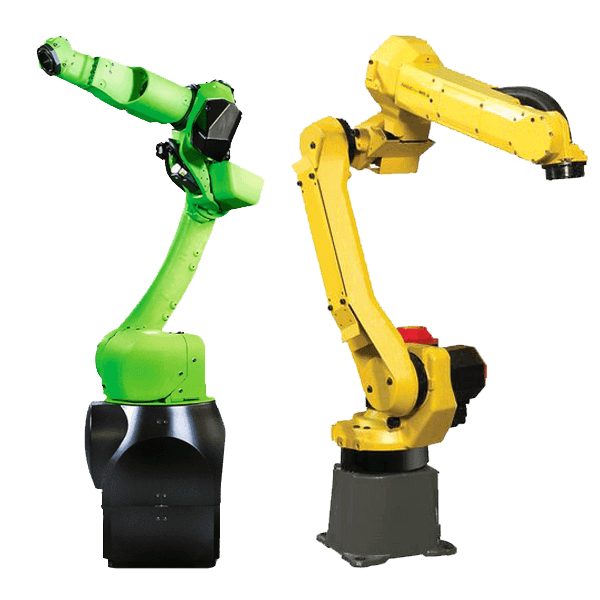
\includegraphics[width=0.75\linewidth]{Images/6-axis-duo.png}
    \caption{Các mẫu cánh tay robot trong công nghiệp}
    \label{fig:enter-label}
\end{figure}

\subsection{Giới thiệu về ngôn ngữ lập trình Python}
Python là một ngôn ngữ lập trình bậc cao, được phát triển bởi Guido van Rossum và lần đầu tiên được phát hành vào năm 1991. Nó nổi bật với cú pháp rõ ràng, dễ đọc và dễ học, giúp lập trình viên có thể phát triển ứng dụng một cách nhanh chóng và hiệu quả.

Các đặc điểm nổi bật của Python:
\begin{itemize}
    \item \textbf{Cú pháp đơn giản:}
    \begin{itemize}
        \item Python có cú pháp gần gũi với ngôn ngữ tự nhiên, giúp người mới bắt đầu dễ dàng tiếp cận.
    \end{itemize}
    \item \textbf{Đa năng:}
    \begin{itemize}
        \item Python có thể được sử dụng cho nhiều mục đích khác nhau, bao gồm phát triển web, phân tích dữ liệu, học máy, trí tuệ nhân tạo, tự động hóa, và nhiều lĩnh vực khác.
    \end{itemize}
    \item \textbf{Thư viện phong phú:}
    \begin{itemize}
        \item Python có một hệ sinh thái thư viện phong phú, bao gồm các thư viện nổi tiếng như NumPy, Pandas, Matplotlib, TensorFlow và Django, giúp lập trình viên dễ dàng thực hiện các tác vụ phức tạp.
    \end{itemize}
    \item \textbf{Hỗ trợ lập trình hướng đối tượng:}
    \begin{itemize}
        \item Python hỗ trợ lập trình hướng đối tượng, cho phép người lập trình tổ chức mã nguồn một cách hiệu quả hơn.
    \end{itemize}
    \item \textbf{Cộng đồng lớn:}
    \begin{itemize}
        \item Python có một cộng đồng lập trình viên lớn và năng động, cung cấp nhiều tài nguyên, hướng dẫn và hỗ trợ.
    \end{itemize}
\end{itemize}

Trong bài tập lớn này sẽ sử dụng Python và các thư viện hỗ trợ sau sau để tạo giao diện và giả lập cánh tay robot:
\begin{itemize}
    \item \textbf{Pygame:}
    \begin{itemize}
        \item Thư viên dùng để vẽ 2-D và tạo animation cũng như tương tác với bàn phím để xoay góc nhìn trong môi trường giả lập cánh tay robot.
    \end{itemize}
    \item \textbf{Numpy:}
    \begin{itemize}
        \item Thư viện Numpy được sử dụng để tính toán các ma trận và một vài phép toán học cơ bản.
    \end{itemize}
    \item \textbf{Matplotlib:}
    \begin{itemize}
        \item Dùng để vẽ đồ thị.
    \end{itemize}
    \item \textbf{Tkinter:}
    \begin{itemize}
        \item Thư viện hỗ trợ tạo giao diện người dùng UI \textit{(User Interface}).
    \end{itemize}
\end{itemize}
\begin{figure}[H]
	\centering
	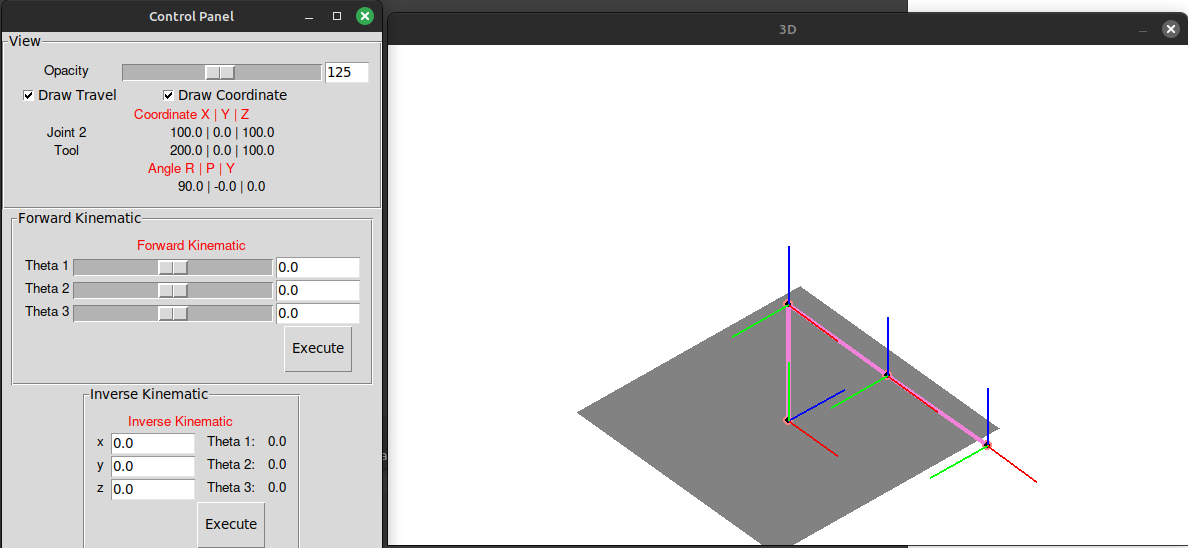
\includegraphics[width=1\linewidth]{Images/software.png}
	\caption{Chương trình được viết bằng Python}
	\label{fig:enter-label1}
\end{figure}
\newpage
\section{ĐỘNG HỌC THUẬN}
\subsection{DH-Table}
\newpage
\section{ĐỘNG HỌC NGHỊCH}
\subsection{Lập công thức giải bài toán động học nghịch}

\subsection{Xây dựng UI và Animation cho bài toán động lực nghịch}
\subsubsection{Giao điện người dùng UI}

Xây dựng giao diện để người dùng nhập tọa độ vị trí của End effector, sau khi bấm nút \textit{Execute} robot sẽ tiến hành di chuyển đến vị trí trên.

\begin{figure}[H]
	\centering
	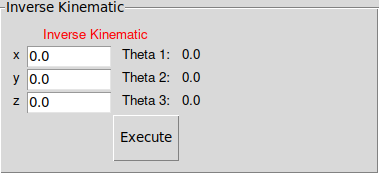
\includegraphics[width=1\linewidth]{Images/inv_ui.png}
	\caption{Giao diện Inverse Kinematic}
	\label{fig:enter-label8}
\end{figure}

\subsubsection{Tạo animation và di chuyển robot theo bài toán động lực nghịch}

Dựa vào các công thức đã lập được ở trên và các giá trị $x$, $y$ và $z$ do người dùng nhập ta tính ngược lại giá trị các góc $\theta_{1}$ , $\theta_{2}$ và $\theta_{3}$, sau khi kiểm tra các góc xaoy có nằm trong phạm vi giới hạn quya của từng khớp ta tiến hành cho robot chuyển động giống như bài toán thuận theo các giá trị $\theta$ vừa tính được ở trên.

\vspace{0.5cm}
\begin{lstlisting}[language=python]
	def inverseKine():
	global guiThetaInv
	px = guiCoorInv[0].get()
	py = guiCoorInv[1].get()
	pz = guiCoorInv[2].get()-d[0]
	# Check valid
	valid = 0
	tmp = (px**2+py**2+pz**2)**0.5
	if (tmp <= a[1]+a[2]) and (tmp >= abs(a[1]-a[2])) and (pz+d[0] >= 0): 
	# calculate
	c3 = (px**2+py**2+pz**2-a[1]**2-a[2]**2)/(2*a[1]*a[2])
	s3 = (1-c3**2)**0.5
	theta3 = atan2(s3, c3)
	
	theta2 = atan2(pz, (px**2+py**2)**0.5) - acos((px**2+py**2+pz**2+a[1]**2-a[2]**2)/(2*a[1]*(px**2+py**2+pz**2)**0.5))
	
	theta1 = atan2(py, px)
	
	valid = 1
	for i, thetaN in enumerate([theta1, theta2, theta3]):
	if thetaN < limitTheta[i][0] or thetaN > limitTheta[i][1]:
	valid = 0
	else: guiThetaInv[i].set(round(thetaN*180/pi, 3))
	
	if valid:
	deltaTime = 60
	nextTheta = np.array([theta1, theta2, theta3])
	stepAngle = np.array([(nextTheta[0]-theta[0])/deltaTime, (nextTheta[1]-theta[1])/deltaTime, (nextTheta[2]-theta[2])/deltaTime])
	animateTranform(nextTheta, stepAngle, deltaTime)
	else:
	tkinter.messagebox.showwarning("Inverse Kinematic.",  "Out of workspace")
\end{lstlisting}

\begin{figure}[H]
	\centering
	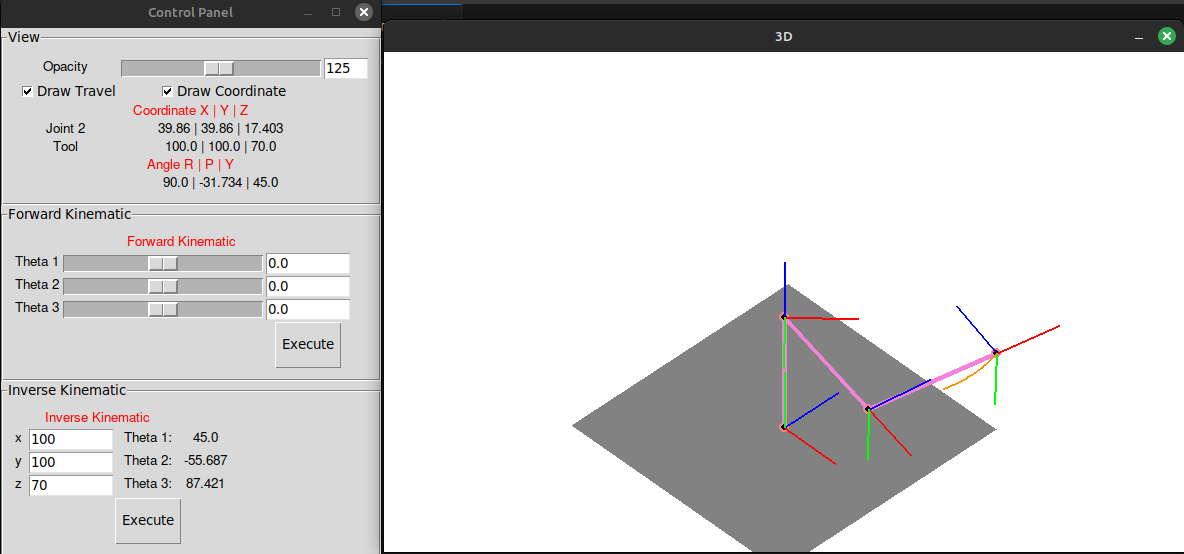
\includegraphics[width=1\linewidth]{Images/inv_demo.png}
	\caption{Inverse Kinematic}
	\label{fig:enter-label9}
\end{figure}
\newpage
\section{QUY HOẠCH QUỸ ĐẠO TRAJECTORY PLANNING}
\subsection{DH-Table}
\newpage
\section{MA TRẬN JACOBI VÀ ĐIỂM KÌ DỊ}
\subsection{DH-Table}
\newpage

\section{ĐÁNH GIÁ CHUNG VÀ KẾT LUẬN}
Sau thời gian thực hiện bài tập lớn môn Nhập môn Kỹ thuật Robot, em có những đánh giá và kết luận chung sau khi hoàn thành bài tập lớn này như sau:
\begin{itemize}
    \item Về những kết quả thu được:
    \begin{itemize}
        \item Biết cách mô phỏng bài toán cũng như kết quả dưới dạng các ứng dụng đơn giản trên nền tảng ngôn ngữ Python 3 bằng cách áp dụng linh hoạt các module cũng như sử dụng các framework hiệu quả.
        \item Hiểu được cấu trúc và những thành phần cơ bản của các bài toán để từ đó xây dựng được các cấu trúc để mô phỏng bài toán. 
        \item Đã hiểu rõ cũng như biết cách áp dụng bài toán động học thuận/nghịch, jacobi vào để giả lập chuyển động robot trong thực tế.
        \item Cải thiện được khả năng lập trình bằng ngôn ngữ Python 3, tận dụng các module sẵn có vô cùng hữu ích của ngôn ngữ này.
    \end{itemize}
    \item Về những hạn chế còn tồn đọng:
    \begin{itemize}
        \item Cải thiện được khả năng lập trình bằng ngôn ngữ Python 3, tận dụng các module sẵn có vô cùng hữu ích của ngôn ngữ này.
    \end{itemize}
\end{itemize}
Qua những đánh giá và kết luận chung như trên, em nhận thấy rằng bản thân đã học thêm được khá nhiều điều mới lạ và đã rèn dũa thêm được những kỹ năng sẵn có. Tuy vậy thì em cũng nhận ra được vẫn còn khá nhiều khuyết điểm quan trọng cần được khắc phục ngay để có thể thực hiện những dự án khác trong tương lai một cách đầy đủ và hoàn thiện hơn. 
\section{VIDEO DEMO VÀ CODE PYTHON}
Link video thuyết trình: \href{}{Nền tảng Youtube}\\
Link slide thuyết trình: \href{}{Nền tảng Canva}
\addcontentsline{toc}{section}{Tài liệu tham khảo}
\begin{thebibliography}{99999}

\bibitem{Robotics}
Bruno Siciliano, Lorenzo Sciavicco, Luigi Villani, and Giuseppe Oriolo. 2008. Robotics: Modelling, Planning and Control (1st. ed.). Springer Publishing Company, Incorporated.

\bibitem{Learning Python}
Mark Lutz. 2009. Learning Python: Powerful Object-Oriented Programming (4th. ed.). O'Reilly Media, Inc.

\end{thebibliography}
\end{document}
